\section*{IV. RESULTS}
\label{sec:results}
\addcontentsline{toc}{section}{IV. \hspace{0.05in} Results}
\hspace{0.25in}
The table in Figure \ref{fig:ethshift} lists the mixtures of ethanol used to test for a change in index of refraction. The graph in Figure \ref{fig:ethshift} shows the different indices of refraction corresponding to mixture A being injected over the interval $[25, 55]$. Similarly mixture B was injected over the interval $[70, 90]$, and mixture C over $[100, 150]$. After the mixtures have time to settle in the chamber, they are flushed out with the same deionized water used to indicate the baseline mode position. Upon injecting a mixture with a higher index into the chamber we notice that the mode position shifts, as expected. Similar tests for mixtures of acetone and 70\% isopropyl alcohol are given in Figures \ref{fig:aceshift} and \ref{isoshift}.

\begin{figure}[h]
\begin{center}
\begin{tabular}{| c c c c |}
	\hline
	Mixtures      	 & A     			  & B      			   & C \\
	\hline
	Ethanol (ml)  	 & 10.\underline{0}   & 20.\underline{0}   & 30.\underline{0} \\
	Water   (ml)  	 & 100.\underline{0}  & 100.\underline{0}  & 100.\underline{0} \\
	Index         	 & 1.338\underline{0} & 1.341\underline{8} & 1.345\underline{0} \\
	Pixel Shift  	 & 80.\underline{0}	  & 135.\underline{0}  & 245.\underline{0} \\
	Change in Index  & 0.004\underline{9} & 0.005\underline{2} & 0.011\underline{9} \\   
	\hline
\end{tabular}
	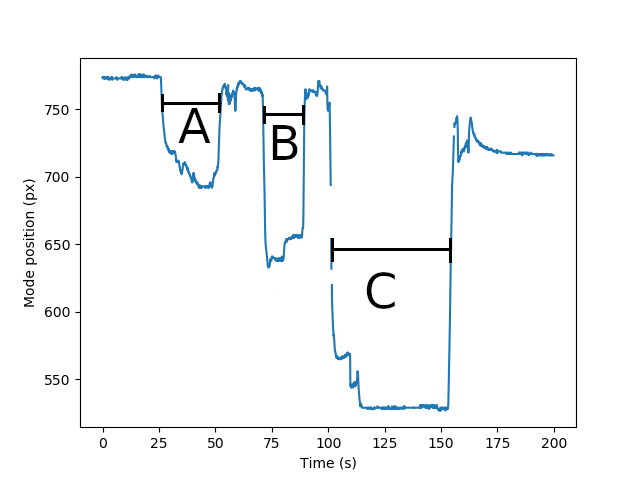
\includegraphics[width=4in]{annotated_mode_4-1-2019}
	\caption{Index shift measurements for ethanol.}
	\label{fig:ethshift}
\end{center}
\end{figure}

\hspace{0.1in}
Using this data we can acquire a value of an index shift per pixel shift to quantify the sensitivity of the sensor. All of the mixtures used for testing have indices between 1.3380 and 1.3464, meaning that when the pixel shift of each mixture is plotted against the index of each we should expect a linear graph (see Figure \ref{fig:modevsindex}) since small variations in reflected angle will yield a proportional shift in pixels.
By extrapolating the data provided in Figure \ref{fig:pxshiftvsindexshift} we that a shift in one pixel corresponds to a shift of about 0.0018 in index of refraction. This level of sensitivty the exceeds the necessary sensitive to detect surface loading.

\begin{figure}
\begin{center}
\hskip+2.5cm\begin{tabular}{| c c c c |}
		\hline
		Mixtures      	 & A     			  & B      			   & C \\
		\hline
		Acetone (ml)  	 & 10.\underline{0}   & 20.\underline{0}   & 30.\underline{0} \\
		Water   (ml)  	 & 100.\underline{0}  & 100.\underline{0}  & 100.\underline{0} \\
		Index         	 & 1.338\underline{4} & 1.343\underline{0} & 1.346\underline{4} \\
		Pixel Shift  	 & 111.\underline{5}  & 206.\underline{0}  & 292.\underline{5} \\
		Change in Index  & 0.005\underline{2} & 0.009\underline{8} & 0.013\underline{2} \\   
		\hline
	\end{tabular}
	\newline
		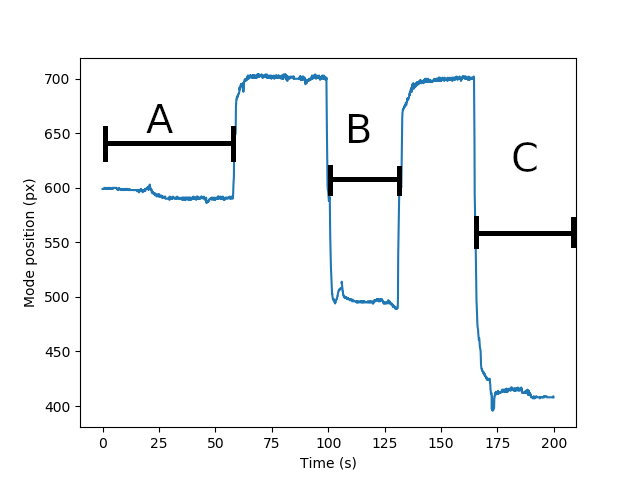
\includegraphics[width=0.6\textwidth]{annotated_acetone_mode.png}
		\caption{\small{Index shift measurements for acetone.}}
		\label{fig:aceshift}
\end{center}
\end{figure}

\vspace{-1.2cm}

\begin{figure}
\begin{center}
\hskip+2.5cm\begin{tabular}{| c c c c |}
		\hline
		Mixtures      	 & A     			  & B      			   & C \\
		\hline
		70\% Isop Alc. (ml)  	 & 10.\underline{0}   & 20.\underline{0}   & 30.\underline{0} \\
		Water   (ml)  	 & 100.\underline{0}  & 100.\underline{0}  & 100.\underline{0} \\
		Index         	 & 1.339\underline{8} & 1.341\underline{2} & 1.344\underline{7} \\
		Pixel Shift  	 & 84.\underline{5}	  & 164.\underline{5}  & 223.\underline{0} \\
		Change in Index  & 0.006\underline{6} & 0.008\underline{0} & 0.011\underline{5} \\   
		\hline
	\end{tabular}
	\newline
		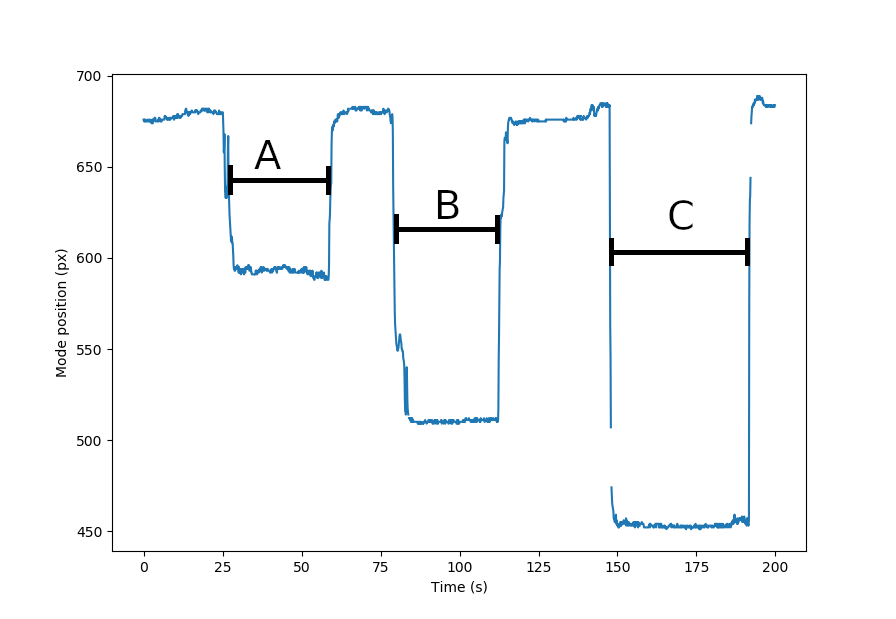
\includegraphics[width=0.6\textwidth]{annotated_isopropal_mode.png}
		\caption{\small{Index shift measurements for 70\% isopropyl alcohol.}}
		\label{isoshift}
\end{center}
\end{figure}

\begin{figure}
	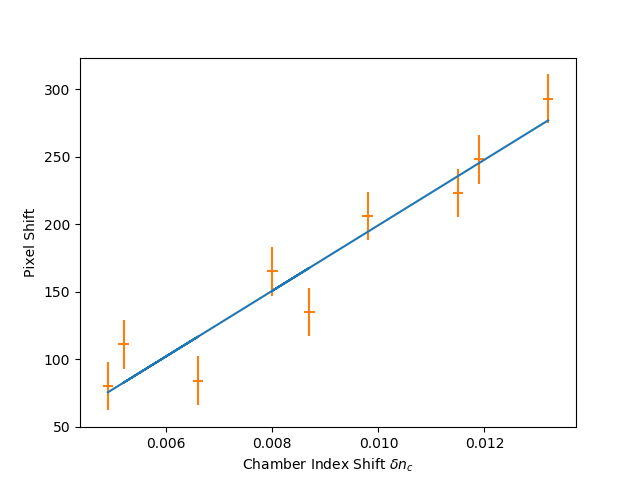
\includegraphics[width=\textwidth]{indexshiftperpx.png}
	\caption{Plotted above is the relationship between a shift in the mode position (measured in pixels) and a shift in the index of refraction of the chamber, $\delta n_c$.}
	\label{fig:pxshiftvsindexshift}
\end{figure}